\documentclass[xcolor={dvipsnames}]{beamer}
\mode<presentation>{\usetheme{boxes}}
\usecolortheme{default}
\setbeamertemplate{navigation symbols}{}%remove navigation symbols

\setbeamerfont{frametitle}{size=\Large}

%\setbeamercolor{structure}{fg=beamer@blendedblue}



\setbeamertemplate{bibliography item}{\insertbiblabel}

\setbeamercolor{bibliography entry author}{fg=black}
\setbeamercolor{bibliography entry title}{fg=black} 
\setbeamercolor{bibliography entry location}{fg=black} 
\setbeamercolor{bibliography entry note}{fg=black}  

\usepackage[style=numeric,sorting=ydnt,maxnames=1,defernumbers=true, firstinits=true]{biblatex}
\renewbibmacro{in:}{}
\ExecuteBibliographyOptions{sorting=ydnt}

%\addbibresource{./jlescSummerSchool_checkpointing.bib}

\makeatother
\setbeamertemplate{footline}
{
  \leavevmode%
  \hbox{%
    %% \begin{beamercolorbox}[wd=.2\paperwidth,ht=2.25ex,dp=1ex]{date in head/foot}%
    %%   \usebeamerfont{date in foot}
    %% \end{beamercolorbox}%
  %%   \begin{beamercolorbox}[wd=.6\paperwidth,ht=2.25ex,dp=1ex, center]{date in head/foot}%
  %%     \usebeamerfont{date in foot}\insertshortdate
  %% \end{beamercolorbox}%
  \begin{beamercolorbox}[wd=\paperwidth,ht=2.25ex,dp=1ex]{date in head/foot}%
    \usebeamerfont{date in foot}\hfill
    {\scriptsize\insertframenumber{}}\hspace*{2ex}
  \end{beamercolorbox}}%
  \vskip0pt%
}
\makeatletter



\usepackage[utf8]{inputenc}
%\usepackage[T1]{fontenc}
%\usepackage[francais]{babel}
\usepackage{hyperref}
\usepackage{url}
\usepackage{pifont}
\usepackage{changepage}
\usepackage{listings}
\lstset{basicstyle=\ttfamily,
  showstringspaces=false,
  commentstyle=\color{black},
  keywordstyle=\color{black}
}

\usepackage{fancyvrb}
\usepackage{multirow}
\usepackage{tabu} 
\usepackage{colortbl}

\usepackage{marvosym}

\usepackage{eurosym}

%\usepackage{gitdags}
\usepackage{comment}

\usepackage{pdfpages}
\setbeamercolor{background canvas}{bg=}


\usepackage{perpage} %the perpage package
\MakePerPage{footnote}



\definecolor{beamer@blendedblue}{RGB}{0,102,204}

\definecolor{beamer@lightgray}{RGB}{238,238,224}


\definecolor{itemorange}{RGB}{255,114,0}


\definecolor{myorange}{RGB}{255,103,0}


\setbeamertemplate{itemize items}[circle]
\setbeamertemplate{itemize subitem}[triangle]


\setbeamercolor{itemize item}{fg=beamer@blendedblue}
\setbeamercolor{itemize subitem}{fg=gray}


\newcommand<>{\Blue}[1]{{\color#2{beamer@blendedblue}#1}}
%\newcommand<>{\Orange}[1]{{\color#2{BurntOrange}#1}}
\newcommand<>{\Orange}[1]{{\color#2{myorange}#1}}
\newcommand<>{\Alert}[1]{{\Orange{\textbf{#1}}}}


\newcommand{\largeskip}{\vspace{0.6cm}}
\newcommand{\hugeskip}{\vspace{1cm}}



\usepackage{tikz}
\usetikzlibrary{%
decorations.pathreplacing,%
decorations.pathmorphing,%
decorations.shapes,%
decorations.text,%
decorations.markings,%
shapes,%
shapes.callouts,%
shadows,%
arrows,
calc,%
positioning,%
chains,%
backgrounds,%
fit, %
fadings}






\tikzset{
    invisible/.style={opacity=0},
    visible on/.style={alt={#1{}{invisible}}},
    alt/.code args={<#1>#2#3}{%
      \alt<#1>{\pgfkeysalso{#2}}{\pgfkeysalso{#3}} % \pgfkeysalso doesn't change the path
    },
}


\tikzset{
    colornode/.style={
        outer sep=0pt, fill=#1!67, %text height=2ex, text depth=.5ex
    },
    cpu/.style={
        diamond, fill=gray!30, aspect=3, name=CPU#1,
        node contents={$\text{CPU}_{#1}$},
    },
    thread/.style={fill=#1!67,
        minimum width=5ex, minimum height=1.25em},
    tick/.style={very thin},
}



\newcommand{\email}[1]{\href{mailto:#1}{\nolinkurl{#1}}}

\newcommand{\xmark}{\ding{55}}


\AtBeginPart{
  %\frame{\partpage}
  \frame{
    \frametitle{Agenda}
    \small
    \tableofcontents[part=\insertpartnumber,
    sectionstyle=show,
    subsectionstyle=hide,
    subsubsectionstyle=hide]
  }
}

\AtBeginSection[]
{
  \begin{frame}
    \frametitle{Agenda}
    \small
    \tableofcontents[
    sectionstyle=show/shaded,
    subsectionstyle=show/show/hide,
    subsubsectionstyle=hide]
  \end{frame}
}

\AtBeginSubsection[]{
  \mode<presentation>{
    \frame{\tableofcontents[
      sectionstyle=show/hide,
      subsectionstyle=show/shaded/hide,
      subsubsectionstyle=show/show/hide]
    }
  }
}


\date[\the\year]{\the\year}

\newcommand{\shellcmd}[1]{\indent\indent\texttt{\footnotesize\$ #1}}


\title[]{Cloud Computing}
\subtitle{Intégration Continue\footnote{Adapté du cours DevOps de Thomas ROPARS (cf dernier slide)}}

\author[]{\\Danilo Carastan dos Santos
  \\ \vspace{0.5cm} \email{danilo.carastan-dos-santos@univ-grenoble-alpes.fr}}

\definecolor{mybrown}{RGB}{205,133,63}
\definecolor{myblue}{RGB}{28,134,238}

\let\Red=\alert
\newcommand<>{\green}[1]{{\color#2{green!70!black}#1}}
\newcommand<>{\blue}[1]{{\color#2{blue!100!black!100}#1}}
\definecolor{darkgreen}{rgb}{0,0.5,0}

\newcommand\myvdots{{\smash[b]\strut\smash[t]\vdots}}


\usepackage{boxedminipage}
\newenvironment{boitecode}[1]{
    \begin{boxedminipage}{\linewidth}      
%\begin{beamerboxesrounded}[shadow=true,lower=lightex,upper=medex]{#1}
    #1
    \begin{semiverbatim}
}{   \end{semiverbatim}\vspace{-1.5\baselineskip}
    \end{boxedminipage}
%  \end{beamerboxesrounded}
}


\begin{document}


\begingroup
\setbeamercolor{titlelike}{bg=beamer@lightgray, fg=black}
\begin{frame}
\titlepage
\end{frame}

\endgroup



\section{Introduction}


\begin{frame}{DevOps}
  
  \begin{block}{Définition (simple)}
    Ensemble de techniques et d'outils facilitant le passage du
    développement à la production.
  \end{block}

  \bigskip
  \begin{block}{Bien plus que ça:}
    \begin{itemize}
    \item Modèle de fonctionnement de l'entreprise
      \begin{itemize}
      \item Impliquant tous les maillons de la chaîne (RHs, finances, etc.)
      \end{itemize}
    \item Modèle d'interactions entre les équipes
    \item Intégration du retour sur expérience
    \item Une ``culture''
    \end{itemize}
  \end{block}

  %% \begin{center}
  %%   \Alert{Nous en resterons à la définition simple}
  %% \end{center}
  
\end{frame}



\begin{frame}{DevOps}


  Relation entre \Blue{Dev} et \Blue{Ops}:
  \begin{itemize}
  \item \Blue{Dev}: Équipes de développeurs logiciels
  \item \Blue{Ops}: Équipes en charge de la mise en production des
    produits
  \end{itemize}

  \largeskip

  
  Antagonisme fort:
  \begin{itemize}
  \item \Blue{Dev}: Modifications aux moindres coûts, le plus rapidement
    possible
  \item \Blue{Ops}: Stabilité du système, qualité
  \end{itemize}

  \bigskip

  \begin{center}
    \Alert{L'automatisation} est au c\oe{}ur de l'approche DevOps
  \end{center}
  
\end{frame}


\begin{frame}{DevOps: Automatisation}

  \begin{block}{Intégration continue}
    Une méthode de développement logiciel dans laquelle le logiciel
    est reconstruit et testé à chaque modification apportée par un
    programmeur.
  \end{block}

  \begin{block}{Livraison continue}
    La livraison continue est une approche dans laquelle l'intégration
    continue associée à des techniques de déploiement automatiques
    assurent une mise en production rapide et fiable du logiciel.
  \end{block}

  \begin{block}{Déploiement continu}
    Le déploiement continu est une approche dans laquelle chaque
    modification apportée par un programmeur passe automatiquement
    toute la chaîne allant des tests à la mise en production. Il n'y a
    plus d'intervention humaine.
  \end{block}

\end{frame}


\section{Intégration continue}

\begin{frame}{Contexte}
  \framesubtitle{Figure de P. Kemp / P. Smith}

  Cycle de développement logiciel
  \begin{itemize}
  \item Modèle de base en cascade
    \begin{itemize}
    \item Exigences bien définies initialement
    \end{itemize}
  \item Peut être bien adapté pour des logiciels critiques (avion,
    centrale nucléaire, \ldots)
  \end{itemize}

  \begin{center}
    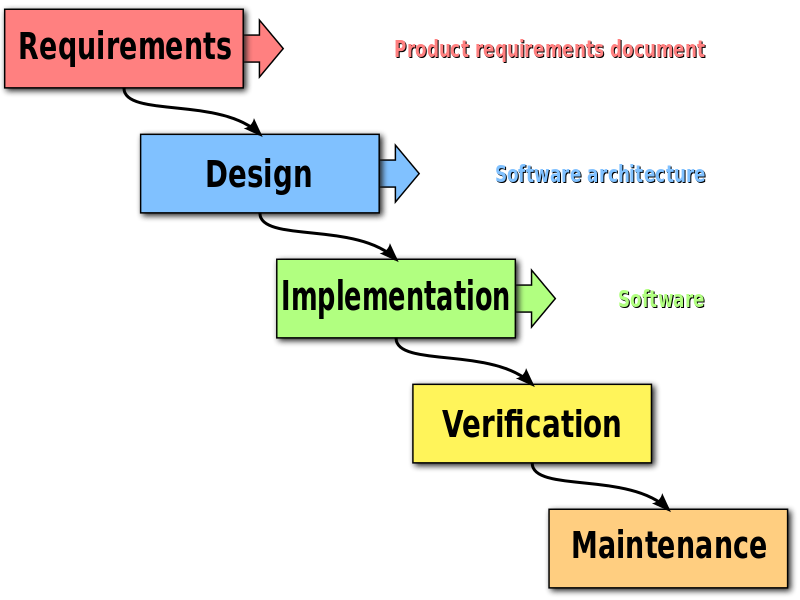
\includegraphics[width=.55\linewidth]{./images/800px-Waterfall_model.png}
  \end{center}
  
\end{frame}


\begin{frame}{Agile}

  Inadapté aux entreprises agiles (startups):
  \begin{itemize}
  \item Contexte turbulent
  \item Exigences changeantes
  \item Clients inconnus (attente du marché inconnue)
  \end{itemize}

  \medskip
  \begin{block}{Développement agile}
    \begin{itemize}
    \item Extreme Programming
    \item Relation étroite entre le client et l'équipe de dev.
      \begin{itemize}
        \item Développement de scénario
        \item Test Driven Development
          \item Changement de priorité, \ldots 
      \end{itemize}
    %\item Seule la recette finale est mise en production
    \end{itemize}
  \end{block}
  
  
\end{frame}

\begin{frame}{Évolution en schéma}
  \framesubtitle{Figure from \url{https://www.mindtheproduct.com/what-the-hell-are-ci-cd-and-devops-a-cheatsheet-for-the-rest-of-us/}}

  \begin{center}
    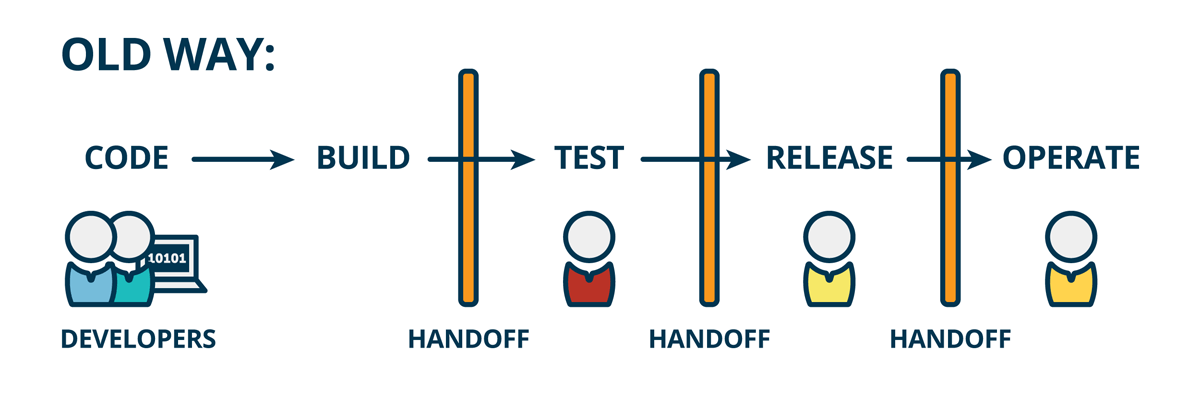
\includegraphics[width=.75\linewidth]{./images/old-way.png}
  \end{center}
  
  \begin{center}
    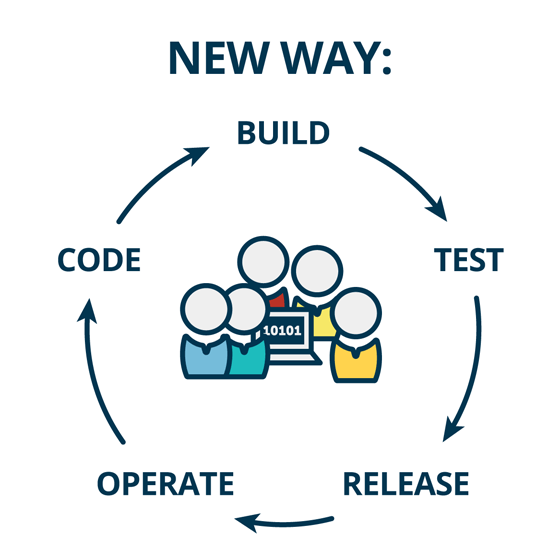
\includegraphics[width=.35\linewidth]{./images/new-way.png}
  \end{center}

\end{frame}




\begin{frame}{L'intégration continue}

  L'intégration continue fait référence à plusieurs pratiques:
  \begin{itemize}
  \item Construire une version fonctionnelle du système chaque jour

    \medskip
  \item Exécuter les tests tous les jours
    \medskip
    
  \item \emph{Committer} ses changements sur le dépôt tous les jours
    \medskip
    
  \item Un système qui observe les changements sur le dépôt et si il
    détecte un changement:
    \begin{itemize}
    \item Récupère une copie du logiciel depuis le dépôt
    \item Compile et exécute les tests
    \item Si les tests passent, possibilité de créer une nouvelle \emph{release} du
      logiciel
    \item Sinon averti le développeur concerné
    \end{itemize}
  \end{itemize}

\end{frame}

\begin{frame}{Pourquoi c'est utile: un exemple}

  Votre chef vous avertit:
  \begin{itemize}
    \item Dans une heure il passe au bureau avec des investisseurs
      pour voir la version la plus récente de votre système.
  \end{itemize}

  \bigskip
  2 scénarios possibles
  \begin{itemize}
  \item Un grand moment de stress qui finit en un échec
    \begin{itemize}
    \item L'état du prototype n'est pas clair, le merge est difficile,
      la démo ne marche pas.
    \end{itemize}
    \medskip

  \item Un non évènement qui se passe sans accroc
    \begin{itemize}
    \item L'état du prototype est clair, la démo se passe sans soucis
    \end{itemize}

  \end{itemize}
  
\end{frame}


\begin{frame}{A propos de l'intégration continue}

  \begin{block}{Avoir un logiciel prêt au déploiement}
    \begin{itemize}
    \item Au début de la phase de développement, le déploiement peut
      sembler lointain
      \begin{itemize}
      \item Ceci peut être source de problèmes
      \end{itemize}

      \medskip
    \item L'intégration continue oblige à avoir un système qui
      fonctionne
      \begin{itemize}
      \item Peut-être qu'il ne fait rien
      \item Ajout des fonctionnalités de manière incrémentale
      \end{itemize}
      
    \end{itemize}
  \end{block}

  %\medskip
  \begin{block}{Échouer au plus tôt}
    \begin{itemize}
    \item Compiler/Tester le système plusieurs fois par jour doit être
      la règle
    \item Détecter les erreurs au plus tôt permet de réagir vite
    \end{itemize}
  \end{block}

\end{frame}

\begin{frame}{A propos de l'intégration continue}

  \begin{block}{Interactions entre équipes de développement}
    \begin{itemize}
    \item Toutes les équipes travaillent sur le même dépôt
    \item L'ensemble des composants logiciels peuvent être testés
      ensemble
      \begin{itemize}
      \item Les problèmes d'intégration sont mis en évidence au plus tôt
      \end{itemize}
    \end{itemize}
  \end{block}

  \begin{block}{Détecter les régressions}
    \begin{itemize}
    \item Une fonctionnalité cesse de fonctionner correctement après
      une modification
    \item Relancer l'ensemble des tests à chaque mise à jour permet de
      détecter efficacement ces problèmes
    \end{itemize}
  \end{block}

  
\end{frame}


\begin{frame}{Un exemple}

  La \emph{disparition} de la société de trading \emph{Knight Capital} 

  \begin{block}{Les faits}
    \begin{itemize}
    \item Société leader dans le \emph{high-frequency} trading
    \item Par erreur, 4 millions de transactions exécutées en quelques
      minutes le 1er Août 2012
    \item Plus de 400M\$ de perte
    \end{itemize}
  \end{block}

  \begin{block}{Les causes}
    \begin{itemize}
    \item Une erreur dans la mise à jour des serveurs de l'entreprise
    \item Échec du code supposé contrôler la validité des transactions
      \begin{itemize}
      \item Code \emph{cassé} lors d'une mise à jour précédente
      \item Pas de tests de régression
      \end{itemize}
    \end{itemize}
  \end{block}
  
\end{frame}


\begin{frame}{Mise en place}

  Pour faire de l'intégration continue, nous avons besoin de:
  \pause
  \begin{itemize}
  \item Un dépôt pour le code source
  \item Un processus de construction automatique du logiciel
  \item Une plateforme pour exécuter des tests
  \end{itemize}

  \bigskip
  Nous avons besoin aussi de:
  \begin{itemize}
  \item Une volonté de travailler de manière incrémentale
  \item Une procédure commune pour envoyer les modifications
  \end{itemize}
  
\end{frame}

\begin{frame}{Procédure d'envoi des modifications}
  
  Tous les développeurs doivent suivre la procédure suivante:
  \begin{enumerate}
  \item Démarrer de la version la plus récente du système
  \item Écrire des procédures de test et faire les changements voulus
  \item Exécuter tous les tests et s'assurer qu'ils passent
  \item Récupérer les dernières modifications depuis le dépôt,
    relancer les tests, et s'assurer qu'ils passent
  \item Envoyer les contributions vers le dépôt
  \end{enumerate}

  \bigskip
  
  À ce moment, les tests d'intégration continue vont être exécutés
  automatiquement.
  
\end{frame}

\begin{frame}{Les outils}

  Les outils que nous pouvons utiliser:

  \begin{itemize}
  \item Un dépôt pour le code source
    \begin{itemize}
    \item svn, git, \ldots
    \item Github
    \end{itemize}
    
    \medskip
  \item Un processus de construction automatique du logiciel
    \begin{itemize}
    \item Make, Ant, Maven \ldots
    \end{itemize}

    \medskip

  \item Une plateforme pour exécuter des tests
    \begin{itemize}
    \item xUnit, JUnit \ldots
    \item Jenkins, Gitlab CI/CD, Github Actions \ldots
    \item Docker
    \end{itemize}

  \end{itemize}
  
\end{frame}




%% \begin{frame}{Outils d'intégration continue}

%%   \begin{block}{Jenkins}
%%     \begin{itemize}
%%     \item Utilisation d'une machine dédiée pour les tests
%%     \item Interface avec différents gestionnaires de version (git) et
%%       builders (Maven).
%%     \end{itemize}
%%   \end{block}


%%   \begin{block}{Travis-CI}
%%     \begin{itemize}
%%     \item \url{https://travis-ci.com/}
%%     \item Intégration continue depuis Github
%%     \item Service gratuit
%%     \end{itemize}
%%   \end{block}
  
%% \end{frame}

%% \begin{frame}{Utilisation de Travis-CI}

%%   \begin{block}{Configuration}
%%     \begin{itemize}
%%     \item Marquer le dépôt à évaluer depuis l'interface web

%%       \medskip
%%     \item Création d'un fichier \texttt{.travis.yml} à la racine du
%%       dépôt
%%       \begin{itemize}
%%       \item Fichier permettant de configurer les tests à exécuter
%%       \end{itemize}

%%       \medskip
%%     \item Cas de Java + Maven
%%       \begin{itemize}
%%       \item Une seule ligne suffit: \texttt{language: java}
%%       \item Si fichier \texttt{pom.xml} présent: exécution de
%%         \texttt{mvn test} 
%%       \end{itemize}
%%     \end{itemize}
%%   \end{block}

%%   \begin{block}{Exécution des tests}
%%     \begin{itemize}
%%     \item Première exécution lors du \emph{push} de
%%       \texttt{.travis.yml}
%%     \item Nouveau test à chaque \emph{push}
%%     \end{itemize}
%%   \end{block}

%% \end{frame}




\section{Livraison continue}


\begin{frame}{Livraison continue}
  \framesubtitle{Continuous Delivery}

  \begin{block}{Définition}
    \begin{itemize}
    \item Optimisation des procédures de livraison de logiciels
      \begin{itemize}
      \item Objectif: Un logiciel doit pouvoir être mis en production
        à tout moment
      \item Les procédures de livraison doivent être automatisées
      \end{itemize}
    \end{itemize}
  \end{block}


  \begin{block}{Motivation}
    \begin{itemize}
    \item La mise en production d'un logiciel est une phase critique
      et complexe
    \item Le faire le plus souvent possible permet de réduire les
      risques et de mieux maîtriser cette procédure
    \item Nécessite un maximum d'automatisation
    \end{itemize}
  \end{block}

\end{frame}


\begin{frame}{Livraison continue et Lean startup}

  \begin{block}{Lean startup}
    \begin{itemize}
    \item \emph{Démarrer maigre}
      \pause
    \item Évaluer l'intérêt d'une fonctionnalité en investissant le
      moins d'effort possible.
    \item Peut s'appliquer aux startups mais aussi aux entreprises
      \emph{classiques}
    \end{itemize}
  \end{block}

  \begin{block}{La livraison continue plutôt que les Releases}
    \begin{itemize}
    \item Dans le modèle \emph{classique}, la mise en production d'une
      nouvelle fonctionnalité se fait lors d'une release
      \begin{itemize}
      \item Les releases ne sont en général pas très fréquentes
      \end{itemize}
    \item La livraison continue permet de mettre de nouvelles
      fonctionnalités rapidement en production 
    \end{itemize}
  \end{block}

\end{frame}

\begin{frame}{Un exemple de Lean startup}
  \framesubtitle{source: A practical guide to continuous delivery}

  \begin{itemize}
    \item Contexte: Un site d'achat en ligne
    \item Nouvelle fonctionnalité: Choisir le jour de livraison d'une
      commande
  \end{itemize}

  \begin{block}{Les étapes}
    \begin{itemize}
    \item Faire de la pub pour la nouvelle fonctionnalité (le
      développement n'a pas commencé)
    \item Si beaucoup de clicks, mettre en oeuvre la fonctionnalité
      (service basique)
      \begin{itemize}
      \item La livraison continue offre un avantage compétitif
      \end{itemize}
    \item Superviser l'utilisation de la nouvelle fonctionnalité
      \begin{itemize}
      \item Imaginer des améliorations pour la fonctionnalité et les
        mettre en production rapidement
      % exemple: les livraisons sont pour des cadeaux d'anniversaire
      % (proposer des suggestions, ajouter un message, etc)
      \end{itemize}
    \end{itemize}
  \end{block}
  
\end{frame}



\begin{frame}{Les étapes de la livraison continue}

  Les étapes principales d'une procédure de livraison continue sont:
  \begin{enumerate}
  \item Commit d'une modification
  \item Exécution des tests unitaires (Intégration continue)
  \item Tests de validation fonctionnelle (acceptance test)
    \begin{itemize}
    \item Tests black-box
    \item Testent si le logiciel répond bien au besoin du client
    \item Peuvent aussi être automatisés
    \end{itemize}
  \item Tests de performances
    \begin{itemize}
    \item Testent si le logiciel peut répondre à la charge
    \item Performance et passage à l'échelle
    \end{itemize}
  \item Tests exploratoires
    \begin{itemize}
    \item Tests non-automatisés effectués par des experts
    \item Exemple: tests d'utilisabilité
    \end{itemize}
  \item Le déploiement en production
  \end{enumerate}

\end{frame}


\begin{frame}{La gestion de l'infrastructure}

  Dans l'approche "livraison continue", la gestion de l'infrastructure
  est elle aussi automatisée.

  \largeskip
  
  \begin{block}{Gestion automatisée}
    \begin{itemize}
    \item La mise en place de l'infrastructure d'exécution est du code
      \begin{itemize}
      \item Géré par le gestionnaire de versions
      \item Décrit les différentes étapes de la mise en place (par ex:
        les logiciels à installer)
      \end{itemize}

      \medskip
      
    \item Des environnements d'exécutions doivent être mis place à
      différentes étapes de la livraison continue
      \begin{itemize}
      \item Pour toutes les phases de test
      \item Pour la mise en production
      \end{itemize}

    \end{itemize}
  \end{block}
  
  
\end{frame}


\begin{frame}{Gestion automatisée de l'infrastructure}
  \framesubtitle{Infrastructure as code}

  \begin{block}{Avantages}
    \pause
    \begin{itemize}
    \item Limite les risques d'erreurs
    \item Assure d'avoir toujours le même environnement d'exécution
    \item Permet de tracer les modifications et de reproduire les
      erreurs
    \item Permet de lier les modifications de l'infrastructure et les
      modifications de l'application
    \item Permet de déployer rapidement un environnement d'exécution
    \end{itemize}
  \end{block}
  
\end{frame}


\begin{frame}{Gestion automatisée de l'infrastructure}
  \framesubtitle{Infrastructure as code}

  \begin{block}{Les outils}
    \begin{itemize}
    \item Docker et les Dockerfile

      \medskip
      
    \item Les outils permettant la configuration d'un environnement
      logiciel (à l'aide de recettes):
      \begin{itemize}
      \item Chef, Puppet, Ansible, etc.
      \end{itemize}

      \medskip
      
    \item Les outils permettant d'approvisionner en ressources (machines
      virtuelles ou conteneurs)
      \begin{itemize}
      \item Vagrant, Terraform, etc.
      \end{itemize}
    \end{itemize}
  \end{block}
  
\end{frame}

\begin{frame}{Minimisation des risques}

  La mise en production est une opération risquée.

  \bigskip
  
  \begin{block}{Minimisation des risques avec la livraison continue}
    \begin{itemize}
    \item Chaque fonctionnalité est mise en production de manière
      indépendante
      \begin{itemize}
      \item Des \emph{petites} mises à jour limitent les risques de problèmes
      \end{itemize}

      \medskip
    \item L'approche \emph{Infrastructure as code} limite les
      mauvaises surprises
      \begin{itemize}
      \item Tests dans les conditions de l'environnement de production
      \item Procédures automatisées
      \end{itemize}
    \end{itemize}
  \end{block}

\end{frame}

\begin{frame}{La mise en production}

  \begin{block}{Quelques remarques}
    \begin{itemize}
    \item Phase critique
    \item Revenir en arrière n'est pas toujours facile
      \begin{itemize}
      \item L'utilisation de gestionnaires de version facilite ce point
      \item Problèmes de retrocompatibilité
        % exemple de données dans une BD dont le format n'est plus le même
      \end{itemize}
    \item Important de faire des \emph{smokes tests} avant une
      utilisation réelle en production
      \begin{itemize}
      \item Vérifier que l'application est démarrée et \emph{fonctionne}
      \end{itemize}
    \end{itemize}
  \end{block}

\end{frame}
  

% Application au lean startup

% Application aux autres entreprises

% Les étapes de livraison en continu (les phases de test)

% La gestion de l'infrastructure

% la minimisation des risques
%% automatisation = toujours la meme chose
%% plus souvent implique moins de modifications à chaque fois

% Les techniques de mise en production

\begin{frame}{Les techniques de mise en production}

  \begin{block}{Canary release}
    
    \begin{itemize}
    \item Rendre disponible une nouvelle version du logiciel à un
      petit sous-ensemble des utilisateurs (10\%):
      \begin{itemize}
      \item Tester en conditions réelles
      \item Avoir un retour sur la nouvelle version (intérêt de
        nouvelles fonctionnalités)
      \item Plusieurs nouvelles versions d'une fonctionnalité peuvent
        être testées en parallèle.
      \item On peut vouloir sélectionner certains clients spécifiques
        pour tester une nouvelle version 
      \end{itemize}
    % \item Applicable en dehors des applications "\emph{serveurs}"
    \end{itemize}
  \end{block}

\end{frame}

\begin{frame}{Les techniques de mise en production}
  
  \begin{block}{Blue-Green deployment}
    \begin{itemize}
    \item Avoir deux environnements de production actifs en même
      temps (Bleu et Vert), un seul est utilisé.
    \item Déploiement et derniers tests du nouveau logiciel sur
      l'environnement non utilisé
    \item Changement de version active en changeant le routage des
      requêtes.
      \begin{itemize}
      \item Changement de version très rapide
      \item Retour en arrière facile
      \end{itemize}
    \end{itemize}
  \end{block}
  
\end{frame}


\begin{frame}{Résumé intégration/livraison/déploiement continu}
  \framesubtitle{Figure by Shahin et al.}
  
  \begin{center}
    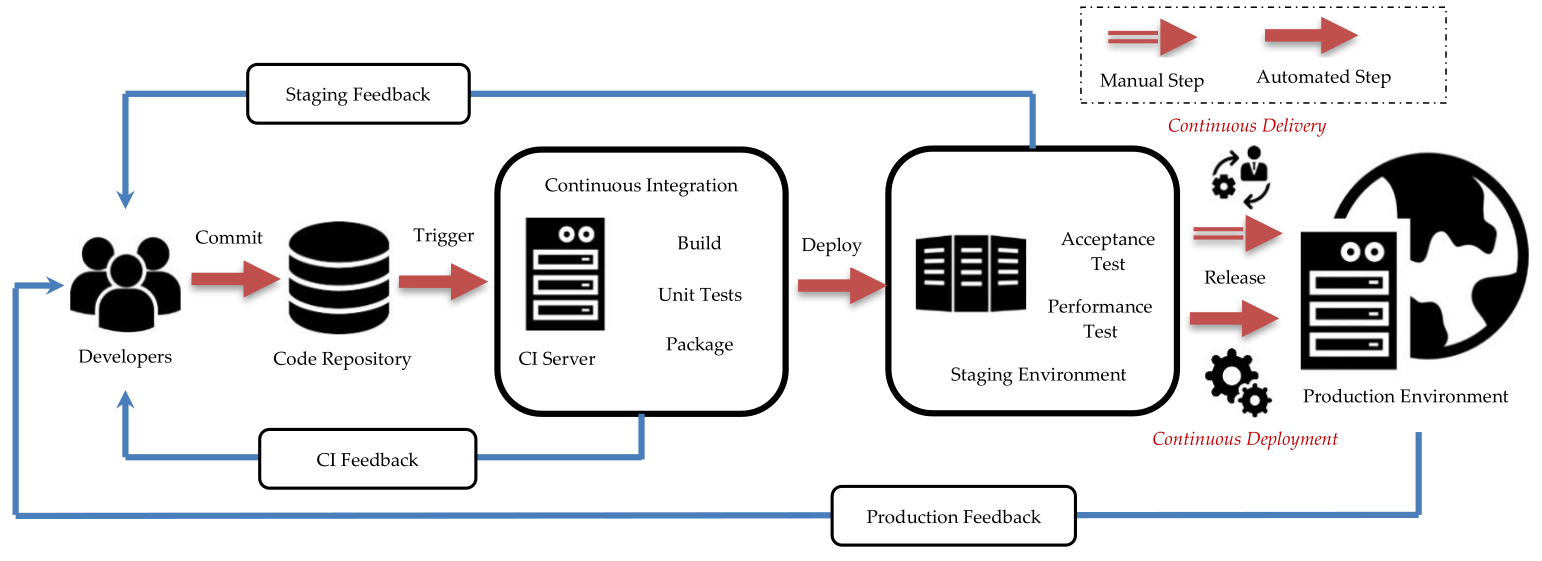
\includegraphics[width=1.1\linewidth]{./images/CI-CD-CD.png}
  \end{center}

  
  
  
\end{frame}



\begin{frame}{Workflow de CD et Docker}
  \framesubtitle{Figure by Zhan et al.}


  \begin{center}
    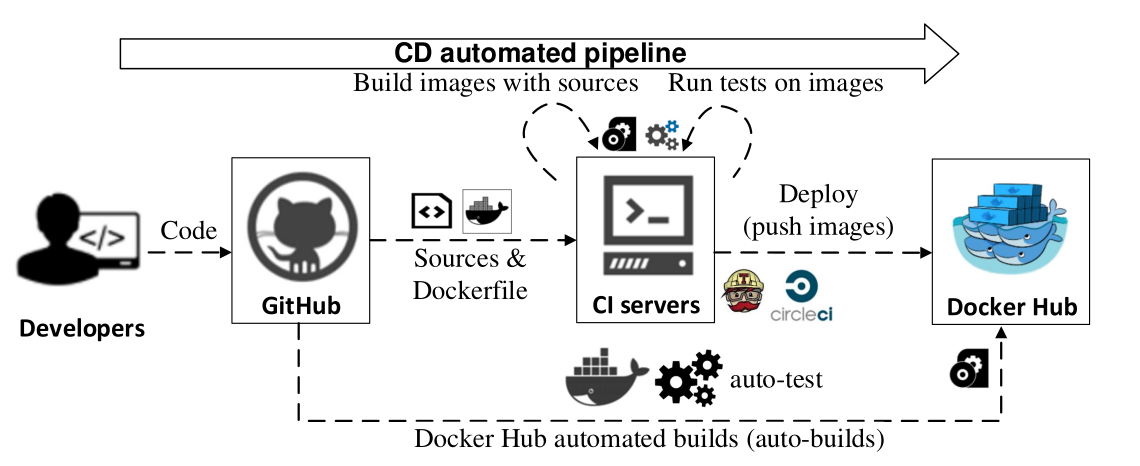
\includegraphics[width=\linewidth]{./images/docker_ci.png}
  \end{center}

  \begin{block}{2 options}
    \begin{itemize}
    \item L'outil de CI/CD publie une nouvelle image quand les tests
      passent avec succès
    \item Dockerhub surveille votre dépôt pour construire une nouvelle
      image lorsqu'il y a des modifications.
    \end{itemize}
  \end{block}
  

\end{frame}


\section{Pipeline de CI/CD}

\begin{frame}{Support CI/CD avec Github ou Gitlab}

  \begin{block}{Fonctionnement similaire offert par Github et Gitlab}
    \begin{itemize}
    \item Définition d'un pipeline d'intégration/livraison continu
    \item Définition à partir d'un fichier Yaml
      \begin{itemize}
      \item Gitlab: Fichier \texttt{gitlab-ci.yml} à la racine du
        dépôt
      \item Github: Fichier yaml à stocker dans le répertoire \texttt{.github/workflows/}
      \end{itemize}
    \end{itemize}
  \end{block}


  \begin{block}{Points d'entrée pour la documentation}
    \begin{itemize}
    \item Gitlab: \url{https://docs.gitlab.com/ee/ci/quick_start/}
    \item Github: \url{https://docs.github.com/en/actions/learn-github-actions/introduction-to-github-actions}
    \end{itemize}
  \end{block}

\end{frame}

\begin{frame}{Les concepts principaux}

  \begin{itemize}
  \item Un \Blue{workflow} (pipeline) est une procédure automatisée
    associée à votre dépôt.

    \medskip
    
  \item Un workflow est composé de un ou plusieurs \Blue{jobs}
    \begin{itemize}
    \item Les jobs peuvent s'exécuter en parallèle par défaut
    \item Possibilité de définir des dépendances entre les jobs
      (Concept de \Blue{stage})
    \end{itemize}

        \medskip

  \item Un job est composé de \Blue{steps} (étapes)
    \begin{itemize}
    \item Une étape est une action/commande
    \end{itemize}

  \end{itemize}

\end{frame}

\begin{frame}{Les concepts principaux (suite)}

  \begin{itemize}
    
  \item Un job est exécuté par un \Blue{Runner}
    \begin{itemize}
    \item Un Runner est un agent en charge d'exécuter un job sur un serveur
      \begin{itemize}
      \item Gitlab/Github fournissent des Runners (et les ressources pour les exécuter)
      \item On peut aussi héberger ses Runners
      \end{itemize}
    \item Les jobs d'un workflow sont exécutés dans des contexte d'exécutions différents
      \begin{itemize}
      \item Les jobs ne peuvent pas partager de données par défaut
      \item Sur les Runners partagés de Gitlab, les jobs s'exécutent dans des conteneurs Docker
      \end{itemize}
    \end{itemize}
    
    \medskip
    
  \item Des \Blue{events} déclenchent le lancement d'un workflow
  \end{itemize}

  
\end{frame}


\begin{frame}{Exemple de workflow Gitlab}

  \begin{center}
    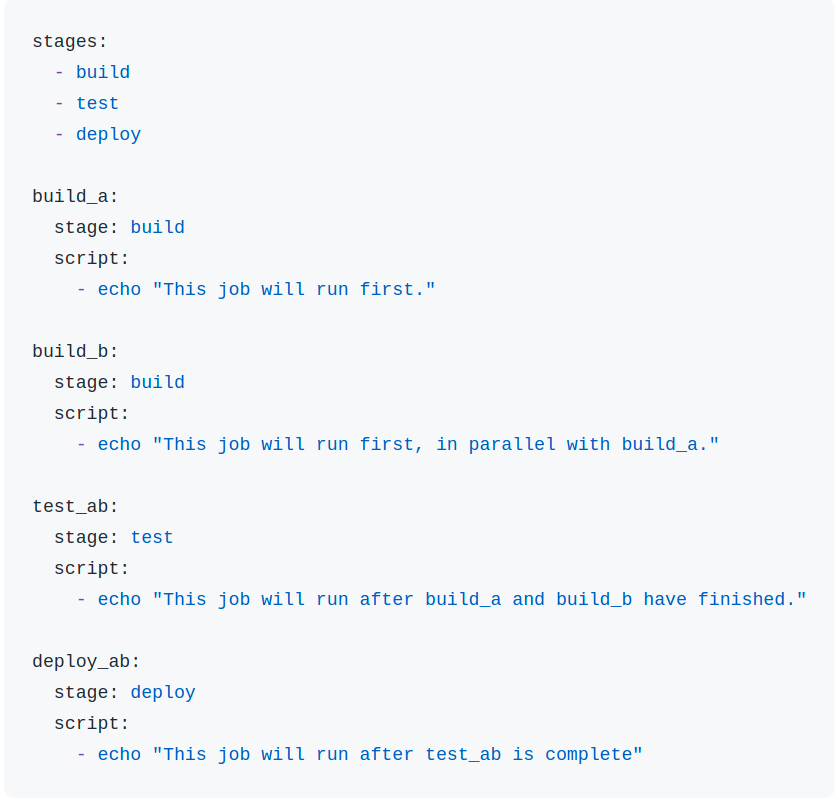
\includegraphics[width=.8\linewidth]{./images/gitlab_pipeline.png}
  \end{center}
  
  
\end{frame}

\begin{frame}{Exemple de workflow Gitlab}

  \begin{block}{Commentaires sur le workflow précédent}
    \begin{itemize}
    \item Les jobs sont associés à des \emph{stages} pour définir des
      dépendances
      \begin{itemize}
      \item L'ordre de déclaration des \emph{stages} définit l'ordre dans lequel elles sont exécutées
      \end{itemize}

      \medskip
      
    \item Les job sont: \texttt{build\_a}, \texttt{build\_b},
      \texttt{test\_ab}, etc.
      \begin{itemize}
      \item Les jobs sont exécutés dans des contextes d'exécution indépendants
      \end{itemize}

      \medskip

      
    \item Les \emph{steps} sont définies sous la balise \texttt{script}
    \end{itemize}
  \end{block}
  
\end{frame}

\begin{frame}{Même exemple avec Github}
\framesubtitle{\url{https://docs.github.com/en/actions/learn-github-actions/migrating-from-gitlab-cicd-to-github-actions}}

  
  \begin{center}
    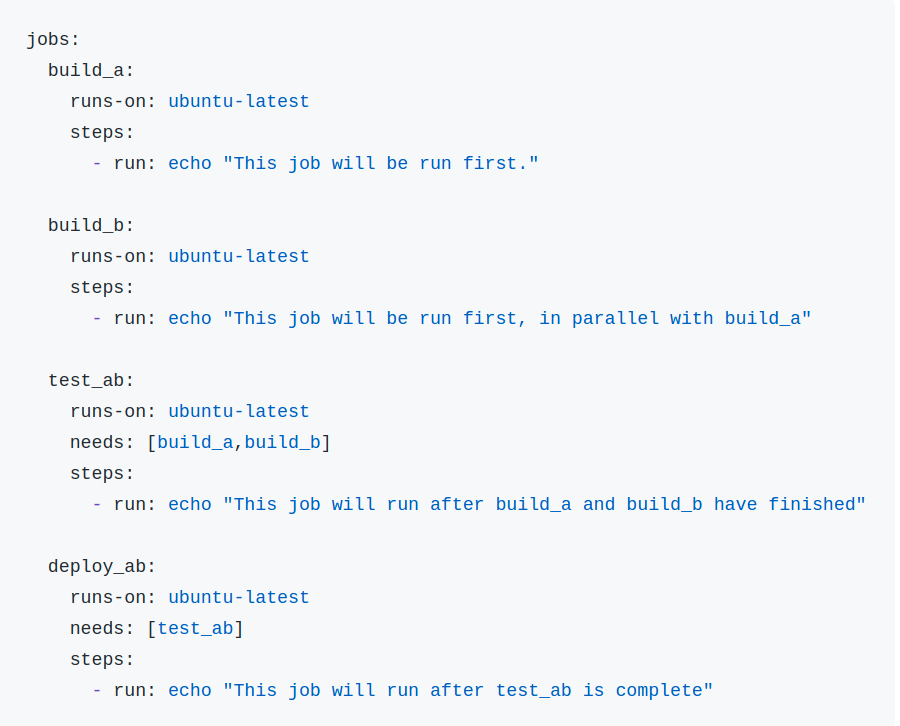
\includegraphics[width=.8\linewidth]{./images/github_pipeline.png}
  \end{center}
  
  
\end{frame}


\begin{frame}{Spécifier une image Docker à utiliser pour un job}

  \begin{center}
    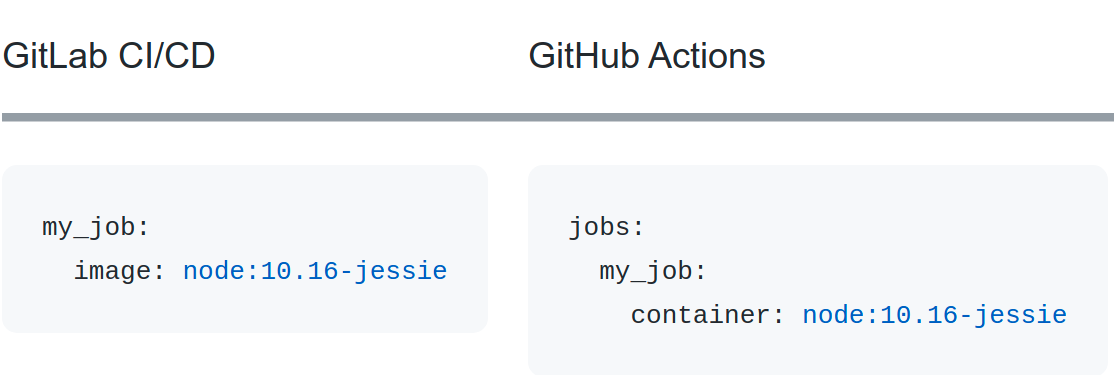
\includegraphics[width=.8\linewidth]{./images/job_docker.png}
  \end{center}


  
\end{frame}


%% \begin{frame}{Toujours plus agile}

%%   \begin{block}{Livraison agile}
%%     \begin{itemize}
%%     \item Lean Startup (Eric Ries)
%%     \item Mettre continuellement en production les nouvelles
%%       fonctionnalités
%%       \begin{itemize}
%%       \item Tester celles-ci auprès de la clientèle (le "marché")
%%       \end{itemize}
%%       \item Mesurer l'intérêt ou le désintérêt de la clientèle
%%       \item Apprendre
%%       \item Persévérer/Améliorer ou Changer de cap
%%     \end{itemize}
%%   \end{block}
  

%% \end{frame}





%% \begin{frame}{Livraison en continue}
%%   \framesubtitle{Continuous Delivery}

%%   \begin{itemize}
%%     \item Automatiser le passage de nouvelles fonctionnalités en test,
%%       pré-production, puis production.

%%       \medskip
%%     \item Automatiser le retour en arrière en cas de besoin (crash,
%%       SLA non respecté, \ldots)
%%   \end{itemize}


%% \end{frame}

%% \begin{frame}{Livraison en continue}
%%   \framesubtitle{Continuous Delivery}


%%   \begin{block}{Techniques associées}

%%     \begin{itemize}
%%     \item Canary release: Rendre disponible une nouvelle version du
%%       logiciel à un petit sous-ensemble des utilisateurs (10\%):
%%       \begin{itemize}
%%       \item Tester en conditions réelles
%%       \item Avoir un retour sur la nouvelle version
%%       \end{itemize}

%%       \bigskip
%%     \item Blue-Green deployment:
%%       \begin{itemize}
%%       \item Avoir deux environnements de production actifs en même
%%         temps (Bleu et Vert), un seul est utilisé.
%%       \item Déploiement et derniers tests du nouveau logiciel sur
%%         l'environnement non utilisé
%%       \item Changement de version active en changeant le routage des
%%         requêtes.
%%       \item Retour en arrière facile
%%       \end{itemize}
%%     \end{itemize}

%%   \end{block}

  

%% \end{frame}

%% \begin{frame}{Livraison en continue}
%%   \framesubtitle{Figure de G. Detrèz}


%%   \begin{center}
%%     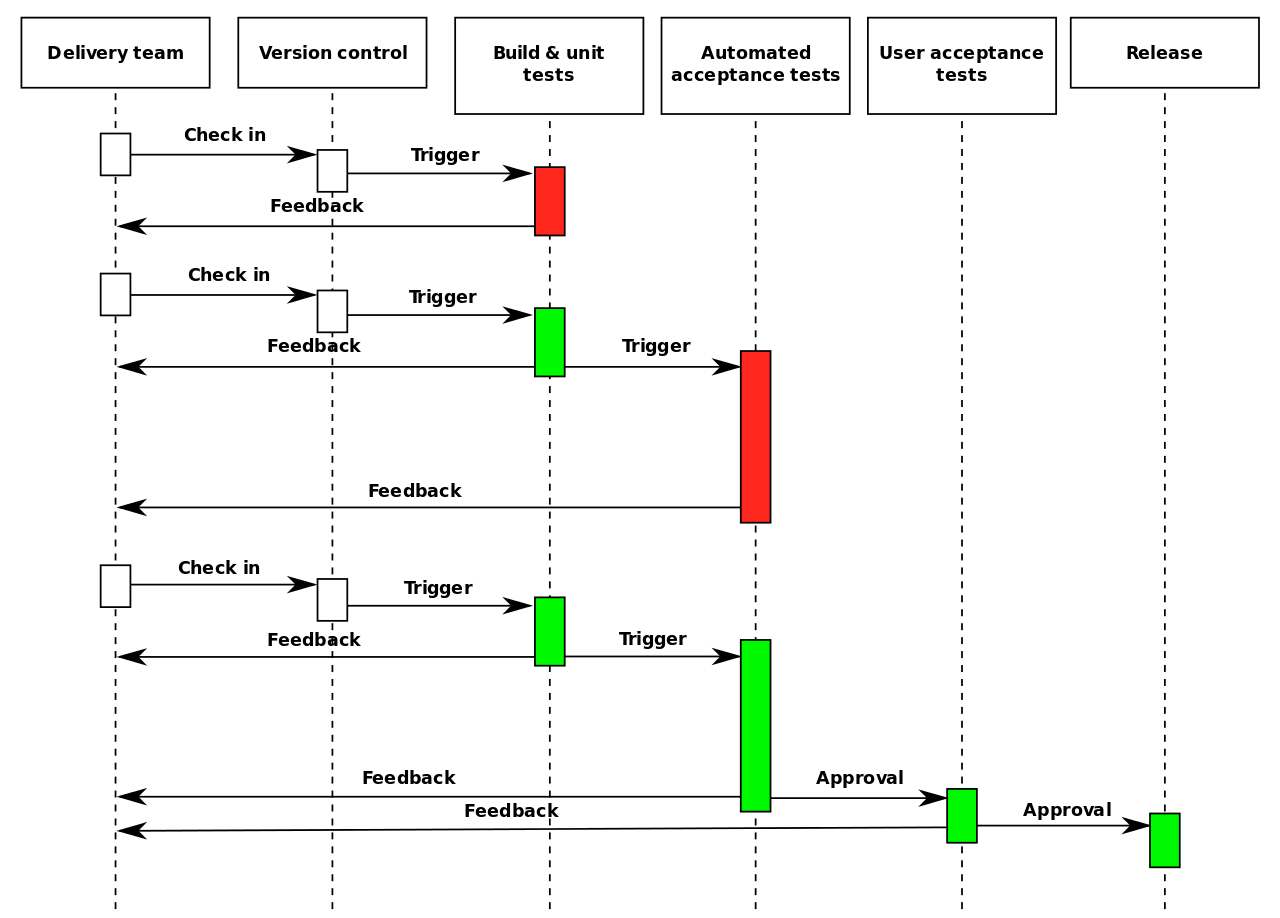
\includegraphics[width=1\linewidth]{./images/Continuous_Delivery_process_diagram.png}
%%   \end{center}
  
%% \end{frame}


\section{Mesures de performance}

\begin{frame}{Mesurer l'impact de l'intégration/déploiement continu}

  Mettre en place des processus de CI/CD peut avoir un coût important
  
  \begin{itemize}
  \item Comment évaluer l'impact sur la qualité des logiciels/services délivrés?

  \item Comment savoir si on est allé assez loin?

  \item Comment savoir si les procédures fonctionnent bien? sont bien suivies?
    
  \end{itemize}

  \bigskip
  
  \center{\Alert{Il faut des métriques}}
  
  
\end{frame}


\begin{frame}{Metriques DORA}
  \subtitle{(Google) DevOps Research and Assessment (DORA)}

  \pause
  
  \begin{block}{4 métriques}
    \begin{itemize}
    \item \Blue{Fréquence des déploiements}: A quelle fréquence l'équipe livre en production?
    \item \Blue{Délai de mise en production}: Le temps nécessaire à un commit pour arriver en production
    \item \Blue{Taux de déploiements problématiques}: Le pourcentage de déploiments qui causent un problème en production
    \item \Blue{Temps nécessaire à la résolution des problèmes}:
      Combien de temps est nécessaire pour corriger les problèmes qui
      apparaissent en production?
    \end{itemize}
  \end{block}


  \begin{block}{Plus de ressources:}
    \begin{itemize}
    \item Les rapports DORA "state of DevOps''
    \item 2024 ACM computing survey: "DevOps Metrics and KPIs: A Multivocal Literature Review" from Amaro et al
    \end{itemize}
  \end{block}
  
\end{frame}


\begin{frame}{Rapport DORA: Accelerate State of DevOps, 2023}

  \begin{center}
    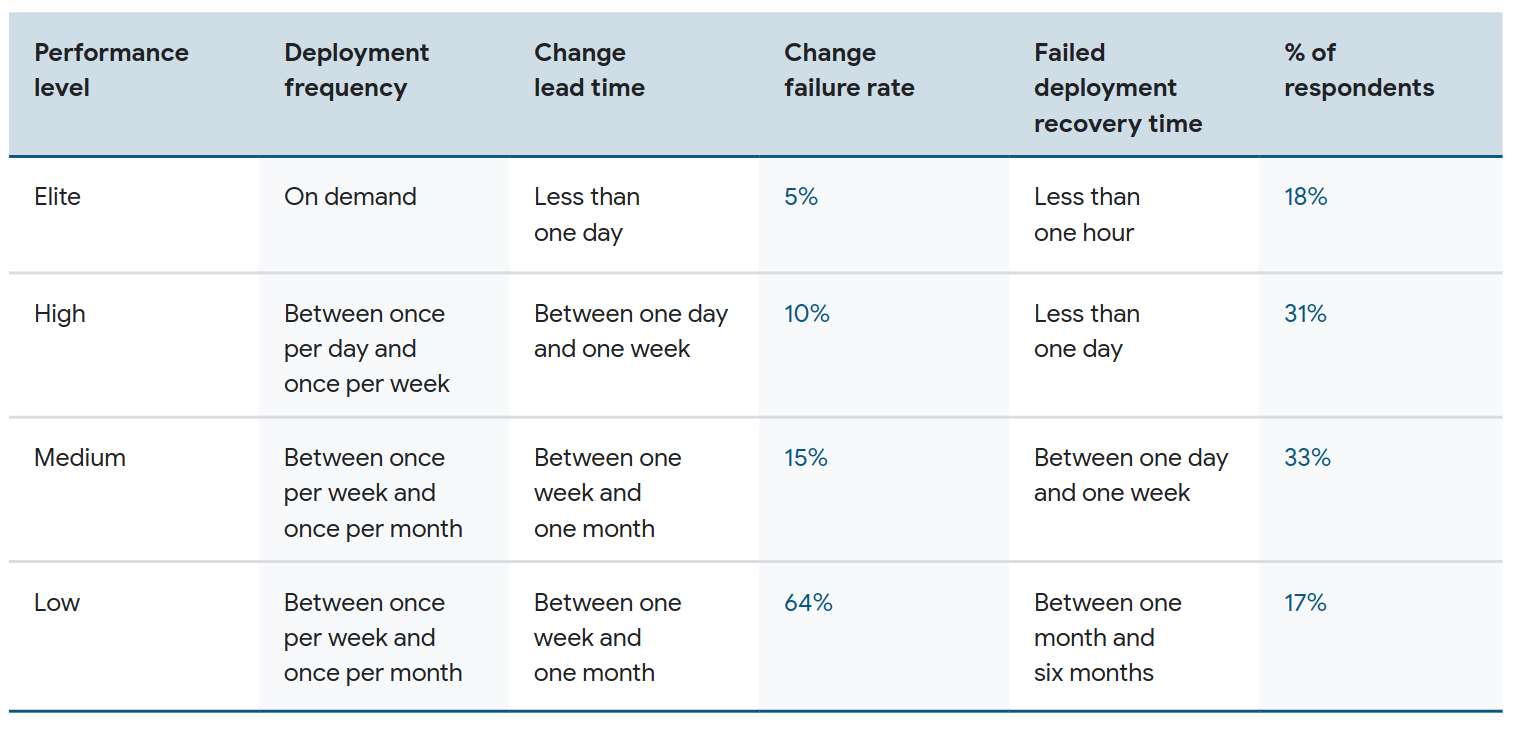
\includegraphics[width=\linewidth]{./images/dora_results.png}
  \end{center}
  

\end{frame}

\begin{frame}{Références}

  \begin{itemize}
  \item Cours DevOps de Thomas Ropars : \url{https://tropars.github.io/teaching/}
  \item Notes de D. Donsez
  \item Notes de K. M. Anderson
  \end{itemize}

  \vspace{1cm}

  \begin{block}{Continuous Delivery (pour aller plus loin)}
  \begin{itemize}
  \item Eric Ries, The Lean Startup: \url{http://theleanstartup.com/}
  \item Dzone Guide To Continuous
  Delivery: \url{https://dzone.com/guides/continuous-delivery-3}
  \item Eberhard Wolff, A practical guide to continuous delivery
  \end{itemize}
  \end{block}

  
\end{frame}




\end{document}
